\begin{frame}{MPS Example: AKLT State}
\vskip-1.5cm
\begin{block}{Haldane Phase for Spin-1 chains $(j=1, m=0)$}
\vskip-0.8cm
$$
H_{AKLT} = \sum\limits_{i} J \vec{S}_i\cdot \vec{S}_{i+1} + J' (\vec{S}_i\cdot \vec{S}_{i+1})^2 + D (S^z_i)^2+BS^x
$$
\end{block}
\begin{columns}[T]
    \begin{column}[T]{.45\textwidth}
        \vskip-1.2cm
        \begin{figure}
        \centering
        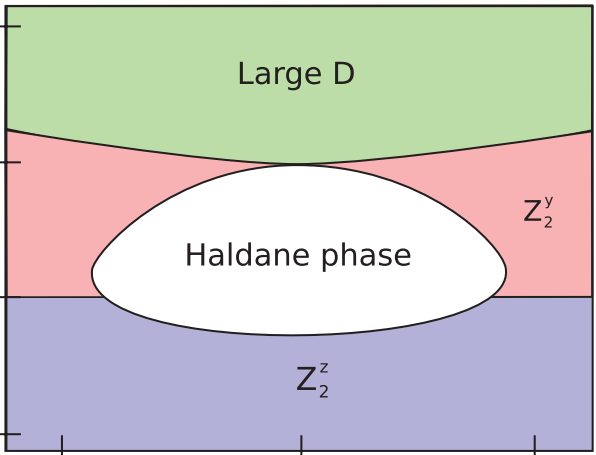
\includegraphics[width=\columnwidth]{diagrams/aklt2.png}
        \end{figure}
    \end{column}
    \begin{column}[T]{.55\textwidth}
    \vskip-0.8cm
    Two distinct featureless insulators:
    \bi 
    \item Large-D phase
    \bi 
    \item Contains product state wavefunction $\ket{\psi} = \ket{000...}$ 
    \ei
    \item Haldane phase
    \bi 
    \item Contains AKLT wavefunction $\ket{\psi} = \Sigma\ket{+00-0+...}$
    \ei 
        \begin{figure}[h]
            \hspace{-2cm}
            \scalebox{1.2}{
            \begin{frame}{MPS Example: AKLT State}
\vskip-1.5cm
\begin{block}{Haldane Phase for Spin-1 chains $(j=1, m=0)$}
\vskip-0.8cm
$$
H_{AKLT} = \sum\limits_{i} J \vec{S}_i\cdot \vec{S}_{i+1} + J' (\vec{S}_i\cdot \vec{S}_{i+1})^2 + D (S^z_i)^2+BS^x
$$
\end{block}
\begin{columns}[T]
    \begin{column}[T]{.45\textwidth}
        \vskip-1.2cm
        \begin{figure}
        \centering
        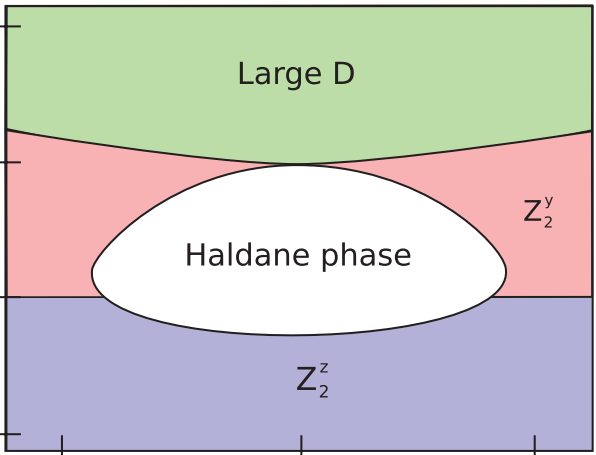
\includegraphics[width=\columnwidth]{diagrams/aklt2.png}
        \end{figure}
    \end{column}
    \begin{column}[T]{.55\textwidth}
    \vskip-0.8cm
    Two distinct featureless insulators:
    \bi 
    \item Large-D phase
    \bi 
    \item Contains product state wavefunction $\ket{\psi} = \ket{000...}$ 
    \ei
    \item Haldane phase
    \bi 
    \item Contains AKLT wavefunction $\ket{\psi} = \Sigma\ket{+00-0+...}$
    \ei 
        \begin{figure}[h]
            \hspace{-2cm}
            \scalebox{1.2}{
            \begin{frame}{MPS Example: AKLT State}
\vskip-1.5cm
\begin{block}{Haldane Phase for Spin-1 chains $(j=1, m=0)$}
\vskip-0.8cm
$$
H_{AKLT} = \sum\limits_{i} J \vec{S}_i\cdot \vec{S}_{i+1} + J' (\vec{S}_i\cdot \vec{S}_{i+1})^2 + D (S^z_i)^2+BS^x
$$
\end{block}
\begin{columns}[T]
    \begin{column}[T]{.45\textwidth}
        \vskip-1.2cm
        \begin{figure}
        \centering
        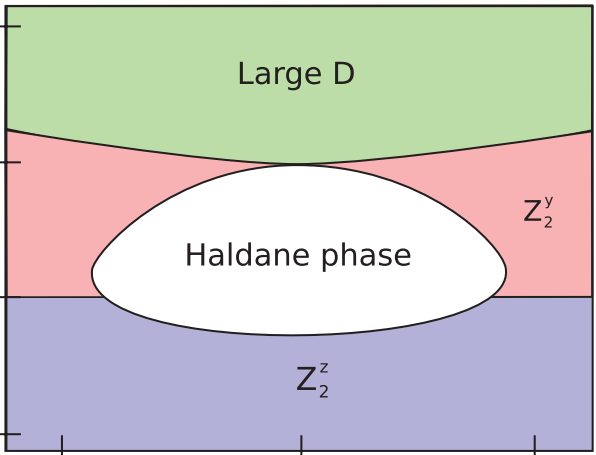
\includegraphics[width=\columnwidth]{diagrams/aklt2.png}
        \end{figure}
    \end{column}
    \begin{column}[T]{.55\textwidth}
    \vskip-0.8cm
    Two distinct featureless insulators:
    \bi 
    \item Large-D phase
    \bi 
    \item Contains product state wavefunction $\ket{\psi} = \ket{000...}$ 
    \ei
    \item Haldane phase
    \bi 
    \item Contains AKLT wavefunction $\ket{\psi} = \Sigma\ket{+00-0+...}$
    \ei 
        \begin{figure}[h]
            \hspace{-2cm}
            \scalebox{1.2}{
            \begin{frame}{MPS Example: AKLT State}
\vskip-1.5cm
\begin{block}{Haldane Phase for Spin-1 chains $(j=1, m=0)$}
\vskip-0.8cm
$$
H_{AKLT} = \sum\limits_{i} J \vec{S}_i\cdot \vec{S}_{i+1} + J' (\vec{S}_i\cdot \vec{S}_{i+1})^2 + D (S^z_i)^2+BS^x
$$
\end{block}
\begin{columns}[T]
    \begin{column}[T]{.45\textwidth}
        \vskip-1.2cm
        \begin{figure}
        \centering
        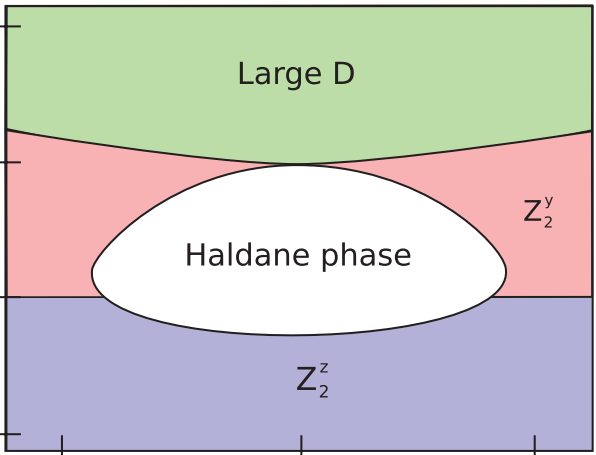
\includegraphics[width=\columnwidth]{diagrams/aklt2.png}
        \end{figure}
    \end{column}
    \begin{column}[T]{.55\textwidth}
    \vskip-0.8cm
    Two distinct featureless insulators:
    \bi 
    \item Large-D phase
    \bi 
    \item Contains product state wavefunction $\ket{\psi} = \ket{000...}$ 
    \ei
    \item Haldane phase
    \bi 
    \item Contains AKLT wavefunction $\ket{\psi} = \Sigma\ket{+00-0+...}$
    \ei 
        \begin{figure}[h]
            \hspace{-2cm}
            \scalebox{1.2}{
            \input{diagrams/aklt.tex}
            }
        \end{figure}

    \ei
    \end{column}
\end{columns}

\end{frame}
            }
        \end{figure}

    \ei
    \end{column}
\end{columns}

\end{frame}
            }
        \end{figure}

    \ei
    \end{column}
\end{columns}

\end{frame}
            }
        \end{figure}

    \ei
    \end{column}
\end{columns}

\end{frame}